% This is an example of a chemistry lab report
% It includes examples of:
	% use of the achemso package to format the report like a proper journal article
	% importing and including a picture file
	% generating in text citations and a bibliography from a bibtex (.bib) file
	% using amsmath, siunitx, and mchem, packages which help writing chemical and mathematical formulas
	% using a tabular environment to create a table of data

% Compiling the .tex, .bib, and .png file can be a little tricky, but the easy way is to simply upload these three files to a new project on overleaf.com, which should automatically compile them into a .pdf


\documentclass[
journal=aamick,
manuscript=article]{achemso}
%\setkeys{acs}{abbreviations=true}
\setkeys{acs}{keywords=true}

\usepackage[version=3]{mhchem} % Formula subscripts using \ce{}
\usepackage{siunitx} % \SI{}{} and \si{} command for typesetting SI units
\usepackage{graphicx} % Required for the inclusion of images
\usepackage{amsmath} % Required for some math elements 
\usepackage{wrapfig}
\usepackage{natbib}

\newcommand*\mycommand[1]{\texttt{\emph{#1}}}
%\providecommand{\e}[1]{\ensuremath{\times 10^{#1}}}
\DeclareSIUnit\molar{\mole\per\gram}
\DeclareSIUnit\Molar{\textsc{m}}

%%%%%%%%%%%%%%%%%%%%%%%%%%%%%%%%%%%%%%%%%%%%%%%%%%%%%%%%%%%%%%%%%%%%%

\author{Amin O. Mesbah}
\email{mesbah.amin@gmail.com}
\affiliation[LACC]{Department of Chemistry, Los Angeles City College, Los Angeles, CA}

%%%%%%%%%%%%%%%%%%%%%%%%%%%%%%%%%%%%%%%%%%%%%%%%%%%%%%%%%%%%%%%%%%%%%

\title[Experiment 03]
{Identification of a Metal Carbonate}

%%%%%%%%%%%%%%%%%%%%%%%%%%%%%%%%%%%%%%%%%%%%%%%%%%%%%%%%%%%%%%%%%%%%%

\abbreviations{Acid Test, Carbonate, Carbon Dioxide, Hydrochloric Acid, Metal, Stoichiometry}
\keywords{Acid Test, Carbonate, Carbon Dioxide, Hydrochloric Acid, Metal, Stoichiometry}

\begin{document}
%%%%%%%%%%%%%%%%%%%%%%%%%%%%%%%%%%%%%%%%%%%%%%%%%%%%%%%%%%%%%%%%%%%%%

\begin{abstract}
In this experiment, a sample of unknown metal carbonate was reacted with hydrochloric acid to produce water and carbon dioxide gas. The mass of the escaping carbon dioxide gas was determined and used to calculate the molar mass of the unknown metal carbonate. This mass was then used to determine the identity of the unknown out of a selection of possibilities. The mean calculated molar mass from three trials was \SI{119.6}{\Molar} with a percent error of less than \SI{5}{\percent}. The unknown metal carbonate was determined to be sodium carbonate hydrate.
\end{abstract}


%%%%%%%%%%%%%%%%%%%%%%%%%%%%%%%%%%%%%%%%%%%%%%%%%%%%%%%%%%%%%%%%%%%%%
%% Start the main part of the manuscript here.
%%%%%%%%%%%%%%%%%%%%%%%%%%%%%%%%%%%%%%%%%%%%%%%%%%%%%%%%%%%%%%%%%%%%%


\section{Introduction}
The purpose of this experiment was to identify an unknown metal carbonate based on the amount of carbon dioxide gas released during a reaction with hydrochloric acid. This technique is known as the "acid test," and is used by geologists to identify carbonate-containing rocks \cite{m}.

The equation of the reaction follows the form:

\begin{equation}
    \ce{M2CO3 + 2HCl -> 2MCl + H2O + CO2}
    \label{eq:carbonate}
\end{equation}

Or, in the case of a bicarbonate (hydrogen carbonate):

\begin{equation}
    \ce{MHCO3 + HCl -> MCl + H2O + CO2}
    \label{eq:bicarbonate}
\end{equation}

During this reaction, water and carbon dioxide are formed. Although carbon dioxide is soluble in water at high pressures, the standard atmospheric pressure of the lab environment allows it to escape as a gas \cite{d}. Through repeated weighing, the mass of the escaped carbon dioxide gas can be determined. Stoichiometry then allows us to determine the moles of the carbon dioxide produced from the reaction.

The balanced equation above shows us that the moles of unknown metal carbonate must equal the moles of released carbon dioxide gas. We use this information, along with the mass of the unknown sample, to determine the molar mass of the unknown. We can then choose from a given selection of 5 possible metal carbonates (Figure \ref{tab:givens}) the one our determined molar mass most closely matches.

\begin{figure}
    \begin{tabular}{|l|l|l|}
        \hline
	        \textbf{Chemical Name} & \textbf{Chemical Formula} & \textbf{Molar Mass (\SI{}{\Molar})}\\
        \hline
	        Sodium Carbonate & \ce{Na2CO3} & 105.99\\
        \hline
	        Sodium Carbonate Hydrate & \ce{Na2CO3 * 1/2H2O} & 114.99\\
        \hline
	        Sodium Bicarbonate & \ce{NaHCO3} & 84.008\\
        \hline
	        Potassium Carbonate & \ce{K2CO3} & 138.21\\
        \hline
	        Potassium Bicarbonate & \ce{KHCO3} & 100.118\\
	    \hline
    \end{tabular}
    \caption{Possible metal carbonates and their molar masses}
    \label{tab:givens}
\end{figure}


\section{Experimental Details}

\subsection{Materials}
%\begin{wrapfigure}{r}{0.5\textwidth}
%\vspace{-230pt}
%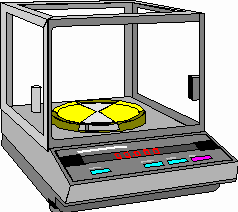
\includegraphics[scale=0.7]{balance}
%\end{wrapfigure}

\vspace{15pt}
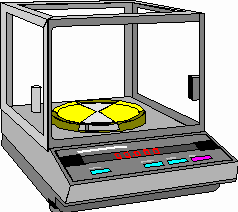
\includegraphics[scale=0.7]{balance.png}
\begin{itemize} \itemsep0pt \parskip0pt \parsep0pt
    \item \SI{4.0}{\Molar}Hydrochloric Acid
    \item Analytical Balance
    \item Erlenmeyer Flask
    \item Graduated Cylinder
    \item Lab Notebook
    \item Paper Towels
    \item Safety Goggles
    \item Styrofoam Cup
    \item Unknown Metal Carbonate Sample
\end{itemize}

\subsection{Safety Considerations}
Hydrochloric acid and some of the metal substances used in this experiment are dangerous and corrosive \cite{c}. I avoided skin contact and was prepared rinse the affected area immediately if contact was made. I made efforts to not inhale corrosive mist from the reaction. I wore safety goggles for the duration of the experiment \cite{a}.

\subsection{Methods}
I first measured \SI{10.0}{\milli\liter} of \SI{4.0}{\Molar}\ce{HCl} in a graduated cylinder and poured it into a styrofoam cup. I weighed a small erlenmeyer flask on an analytical balance, then added approximately \SI{2}{\gram} of of my unknown metal carbonate to the the flask and reweighed it to the nearest \SI{0.0001}{\gram}. I weighed the cup, flask, and sample together, then the cup and acid alone. Back in my work area, I poured the acid slowly into the flask. I waited 5 minutes for the reaction to finish, then blew into the flask to clear the remaining \ce{CO2} gas. Again I weighed the cup, flask, and contents together \cite{b}. After recording all my measurements, I disposed of the flasks contents in a lab sink and rinsed all my materials. I repeated this procedure 2 more times for a total of 3 trials.


\section{Theoretical Basis}
From any balanced chemical equation, we can determine the mole ratios between any reactants or products \cite{e}. For example, from the balanced equation in equation \ref{eq:carbonate} we know that, for a reaction of \ce{M2CO3} with \ce{HCl}, there is \SI{1}{\mole} of \ce{CO2} for every \SI{1}{\mole} of \ce{M2CO3}, and \SI{2}{\mole} \ce{HCl} for every \SI{1}{\mole} \ce{CO2}.

Figure \ref{fig:balEquations} shows the balanced chemical equations for each possible reaction:

\begin{figure}
    \begin{tabular}{l}
    \ce{Na2CO3 + 2HCl -> 2NaCl + H2O + CO2}\\
    \ce{Na2CO3 * 10H2O + 2HCl -> 2NaCl + 11H2O + CO2}\\
    \ce{NaHCO3 + HCl -> NaCl + H2O + CO2}\\
    \ce{K2CO3 + 2HCl -> 2KCl + H2O + CO2}\\
    \ce{KHCO3 + HCl -> KCl + H2O + CO2}\\
    \end{tabular}
  \caption{Balanced chemical equations}
  \label{fig:balEquations}
\end{figure}


The "acid test" in this experiment works because of these mole ratios. We measure the mass of the metal carbonate, then we determine the mass of the \ce{CO2} \cite{f}. Stoichiometry allows us to use these measurements, along with our mole ratios and the known molar mass of \ce{CO2}, to identify the unknown carbonate (represented here as \ce{M2CO3}) by its own molar mass \cite{l}:

\begin{equation}
  \SI{}{\gram}{\ce{CO2}}
  \times \frac{\SI{1}{\mole}\ce{CO2}}{\SI{44.01}{\gram}\ce{CO2}}
  \times \frac{\SI{1}{\mole}\ce{M2CO3}}{\SI{1}{\mole}\ce{CO2}}
  = \SI{}{\mole}{\ce{M2CO3}}
  \label{eq:gtomol}
\end{equation}

\begin{equation}
  \frac{\SI{}{\mole}{\ce{M2CO3}}}{\SI{}{\gram}{\ce{M2CO3}}}
  = \SI{}{\Molar}{\ce{M2CO3}}
  \label{eq:molarity}
\end{equation}

In order to to determine the accuracy of our measurements we can calculate the percent error between our result and the known molar mass of whichever metal carbonate we believe our unknown to be:

\begin{equation}
  \text{\%err.} =
  \frac{|\text{true value}-\text{experimental value}|}{\text{true value}}
  \times 100
  \label{eq:error}
\end{equation}


\section{Results and discussion}
\begin{figure}
    \begin{tabular}{|l|l|l|l|}
        \hline
	         \textbf{Mass} &  \textbf{Trial 1} &  \textbf{Trial 2} &  \textbf{Trial 3}\\
        \hline
	        Empty Flask & 102.5692 & 102.5694 & 102.5685\\
        \hline
	        Empty Cup & 2.2105 & 2.4618 & 2.4683\\
        \hline
	        Flask + Sample & 104.5708 & 104.6971 & 104.7928\\
        \hline
	        Cup + Acid & 13.0347 & 13.3504 & 13.1154\\
        \hline
	        Flask + Sample + Cup + Acid (before reaction) & 117.6056 & 118.0472 & 117.9076\\
        \hline
	        Flask + Contents + Cup (after reaction) & 116.8486 & 117.2619 & 117.0819\\
        \hline
    \end{tabular}
    \caption{Recorded masses (\SI{}{\gram})}
    \label{tab:data}
\end{figure}

Figure \ref{tab:data} shows all the recorded mass measurements I made for each of the three trials. The mass of the empty flask and cup did not fluctuate significantly, though a different cup (with a different mass) had to be used for the second and third trials. The other masses varied slightly, and the results of those variations are discussed below \cite{k}.

\begin{figure}
    \begin{tabular}{|l|l|l|l|}
        \hline
	         \textbf{Value} &  \textbf{Trial 1} &  \textbf{Trial 2} &  \textbf{Trial 3}\\
        \hline
	        Mass Sample (\SI{}{\gram}) & 102.5692 & 102.5694 & 102.5685\\
        \hline
	        Mass \ce{CO2} (\SI{}{\gram}) & 2.2105 & 2.4618 & 2.4683\\
        \hline
	        Moles \ce{CO2} (\SI{}{\mole}) & 104.5708 & 104.6971 & 104.7928\\
        \hline
	        Moles Sample (\SI{}{\mole}) & 13.0347 & 13.3504 & 13.1154\\
        \hline
	        Molar Mass Sample(\SI{}{\Molar})& 117.6056 & 118.0472 & 117.9076\\
        \hline
    \end{tabular}
    \caption{Calculated values}
    \label{tab:calculations}
\end{figure}

Figure \ref{tab:calculations} shows the calculations I did based off of the data in figure \ref{tab:data}. The path from grams, to moles, to molar mass can be seen here. It should be noted that the moles of \ce{CO2} and the moles of sample are equal for each trial because the mole ratio of the reaction is \(1:1\) \cite{i}.

The mean of the three final calculations of the unknown carbonate's molar mass is \SI{119.6}{\Molar} \cite{j}. This was closest to sodium carbonate hydrate (figure \ref{tab:givens}), which had a given molar mass of \SI{114.99}{\Molar}. The percent error was \SI{4.0}{\percent}; accurate enough for confidence in the result. The error likely came from measurement error when using the analytical balance, and from failure to completely remove the heavy \ce{CO2} gas from the inside of the cup before reweighing.

\subsection{Sample Calculations}
Sample calculations for Trial 1 are included below:

\begin{equation}
  m_{sample}
  = m_{flask+sample} - m_{flask}
  = \SI{104.5708}{\gram} - \SI{102.5692}{\gram}
  = \SI{2.0016}{\gram}
  \label{eq:msample}
\end{equation}

\begin{equation}
  m_{\ce{CO2}}
  = m_{before} - m_{after}
  = \SI{117.6056}{\gram} - \SI{116.8486}{\gram}
  = \SI{0.7570}{\gram}
  \label{eq:mco2}
\end{equation}

\begin{equation}
  mol_{\ce{CO2}} = m_{\ce{CO2}} \times \frac{\SI{1}{\mole}\ce{CO2}}{\SI{44.01}{\gram}\ce{CO2}}
  = \SI{0.7570}{\gram} \times \frac{\SI{1}{\mole}\ce{CO2}}{\SI{44.01}{\gram}\ce{CO2}}
  = \SI{1.720e-2}{\mole} = mol_{sample}
  \label{eq:molsample}
\end{equation}

\begin{equation}
  M_{sample} = \frac{m_{sample}}{mol_{sample}}
  = \frac{\SI{2.0016}{\gram}}{\SI{1.720e-2}{\mole}}
  = \SI{116.4}{\Molar}
  \label{eq:molaritysample}
\end{equation}

\begin{equation}
  \text{\%err.}
  = \frac{|\text{true value}-\text{experimental value}|}{\text{true value}} \times 100
  = \frac{|\SI{114.99}{\Molar}-\SI{116.4}{\Molar}|}{\SI{114.99}{\Molar}} \times 100
  = \SI{1.2}{\percent}
  \label{eq:error1}
\end{equation}

\section{Conclusions}
The "acid test" proved to be a viable method of identifying an unknown metal carbonate \cite{h}. Careful measurement of mass before and after reaction, identification of molar ratios from a balanced equation, and calculation of the molar mass of carbon dioxide from the periodic table supplied sufficient information to determine the molar mass of the unknown sample \cite{g}. Careful repetition of the procedure compensated adequately for the various sources of error.

%%%%%%%%%%%%%%%%%%%%%%%%%%%%%%%%%%%%%%%%%%%%%%%%%%%%%%%%%%%%%%%%%%%%%
%% The "Acknowledgement" section can be given in all manuscript
%% classes.  This should be given within the "acknowledgement"
%% environment, which will make the correct section or running title.
%%%%%%%%%%%%%%%%%%%%%%%%%%%%%%%%%%%%%%%%%%%%%%%%%%%%%%%%%%%%%%%%%%%%%
\begin{acknowledgement}

The author would like to thank Richard P. Feynman and Douglas Adams.

\end{acknowledgement}

%%%%%%%%%%%%%%%%%%%%%%%%%%%%%%%%%%%%%%%%%%%%%%%%%%%%%%%%%%%%%%%%%%%%%
%% The appropriate \bibliography command should be placed here.
%% Notice that the class file automatically sets \bibliographystyle\cite{a}
%% and also names the section correctly.
%%%%%%%%%%%%%%%%%%%%%%%%%%%%%%%%%%%%%%%%%%%%%%%%%%%%%%%%%%%%%%%%%%%%%

%\nocite{*}
\bibliography{sources}

\end{document}
